%\part*{Lezione 26/04/2021}
\newpage
\section{\textit{The Holy Grail}}\index{the holy Grail of Nuclear Astrophysics@\textit{The Holy grail of Nuclear Astrophysics}}\label{sec-holy-grail}
La misura della reazione di distruzione del carbonio:
$$\alpha +\ce{^{12}C}\to\ce{^{16}O}+\gamma$$
è di importanza tale da essere stata definita nel 1983 da William Fowler nella sua \textit{Nobel Prize lecture} \textit{\vir{The Holy Grail of Nuclear Astrophysics}}. Se infatti la $3\alpha$ produce carbonio, questa reazione lo distrugge in favore dell'ossigeno\footnote{La $3\alpha$ è conosciuta con un'incertezza del 10\%, ma questo non vale per la $\alpha\, \ce{^{12}C}$ (circa il 20\%).}, dunque lo studio della combinazione dei due processi diviene fondamentale per la stima delle abbondanze di questi elementi, peraltro tra i più presenti nell'universo. Nella nostra galassia, per esempio\footnote{Stime spettroscopiche.}:
\begin{align*}
	&74\%\qquad\;\quad\ce{H} \\
	&24\%\qquad\;\;\ce{^{4}He} \\
	&0.85\%\qquad\ce{^{16}O} \\
	&0.39\%\qquad\ce{^{12}C} \\
	&\dots
\end{align*}
\acc{E} una reazione fondamentale anche per l'innesco del C-\textit{burning} e quindi influenza l'evoluzione\footnote{Infatti, durante H-\textit{burning} in \textit{shell} il nucleo di He è inerte e collassa, fin quando non si raggiungono le temperature per l'innesco del He-\textit{burning} tramite la $3\alpha$; i residui di questo processo sono appunto il carbonio e l'ossigeno che deriva da $\ce{^{12}C}(\alpha,\gamma)\ce{^{16}O}$. Conoscere l'abbondanza di questi elementi determina l'evoluzione successiva.} delle \textit{low} e \textit{high mass stars}. Non solo, questa reazione determina anche l'abbondanza di carbonio e ossigeno nelle popolazioni stellari successive.

\subsection{Studio della reazione} Studiamo\footnote{Facciamo riferimento all'articolo R.J., de Boer et al., Rev. Mod. Phys., 2017, vol.89, n.3, \texttt{DOI:}\doi{10.1103/RevModPhys.89.035007}\articolo{de Boer}.} adesso la combinazione di questa reazione con la $3\alpha$. Usando la stessa notazione di Figura \ref{0422_reaz}:
\begin{align*}
	\tderpar{Y_{\ce{^{12}C}}} &= \frac{1}{3!} Y_{\alpha}^3 \rho^2 N_u^2 \, \mean{\sigma v}_{3\alpha} - Y_\alpha Y_{\ce{^{12}C}} \rho N_u \, \mean{\sigma v}_{\alpha\ce{^{12}C}} \\
	\tderpar{Y_{\ce{^{16}O}}} &= Y_\alpha Y_{\ce{^{12}C}} \rho N_u \, \mean{\sigma v}_{\alpha\ce{^{12}C}} - Y_\alpha Y_{\ce{^{16}O}} \rho N_u \, \mean{\sigma v}_{\alpha\ce{^{16}O}}	
\end{align*}
dove abbiamo tenuto conto anche della reazione di distruzione\footnote{La studieremo successivamente.} dell'ossigeno:
$$\alpha + \ce{^{16}O} \to \ce{^{20}Ne} + \gamma$$
con $\mean{\sigma v}_{\alpha \ce{^{16}O}}\lll \mean{\sigma v}_{\alpha \ce{^{12}C}}$.\\ 
Vediamo come viene modificata l'evoluzione stellare che modellizziamo dividendo:
\begin{enumerate}[a)]
	\item $M\leq 8 M\sol$ \textit{stars}\footnote{Sono quelle che fanno il ramo di AGB e terminano in Nane Bianche.}.\\ 
	Terminato He-\textit{burning}, non riescono a innescare il carbonio e il nucleo di C-O comincia a contrarre; gli strati esterni si espandono e raffreddano e la stella entra nella fase di AGB. La quantità $\mean{\sigma v}_{\alpha\ce{^{12}C}}$ determina il tempo dell'He-\textit{burning}, l'inizio dell'AGB e le abbondanze di carbonio e ossigeno della Nana Bianca che si formerà (e quindi della possibile SN IA che potrebbe esserci).  
	\item $M\geq 8M\sol$ \textit{stars}\footnote{Queste evolvono fino a raggiungere \textit{Core-collapse Supernov\ae}.}.\\ 
	Per queste il He-\textit{burning} dura circa $\ord{6}$ y dunque la $3\alpha$ e la $\alpha\,\ce{^{12}C}$ divengono essenziali per la produzione di energia (e da qui la loro importanza). Negli stati finali (alte temperature e densità) la $\alpha\,\ce{^{12}C}$ non è l'unica reazione che \vir{consuma} $\alpha$; vi sono 3 processi:
	\begin{itemize}
		\item $\alpha + \ce{^{12}C} \to \ce{^{16}O} + \gamma$ 
		\item $\alpha + \ce{^{16}O} \to \ce{^{20}Ne} + \gamma $
		\item $\alpha + \ce{^{22}Ne} \to \ce{^{25}Mg} + n$\\ 
		Questa è una delle principali sorgenti\footnote{Su come avere una certa abbondanza di $\ce{^{22}Ne}$ non è banale discutere.} di neutroni (che tipicamente non sono presenti nelle stelle) ed è quindi essenziale per le catture neutroniche successive che permettono di superare il picco del ferro (processo $s$\index{processo s@processo $s$}\footnote{L'incertezza di questi processi dipende quindi dalla $\alpha \, \ce{^{12}C}$.}).
	\end{itemize} 
	In realtà, negli ultimi processi la $\alpha \, \ce{^{16}O}$ non si attiva per cui prima ci sono altri \textit{burning} (C,O,Ne,Si).
\end{enumerate} 

\paragraph{Risonanza dell'ossigeno} 
In Figura \ref{0426_lv} riportiamo i livelli dell'ossigeno e alcune reazioni di produzione, tra cui $\alpha \, \ce{^{12}C}$. Osserviamo che i dati si fermano a circa 2 MeV mentre l'energia di Gamow è di circa 300 keV, quindi è necessaria la teoria per l'estrapolazione dei risultati.

\begin{figure}[h]
	\centering
	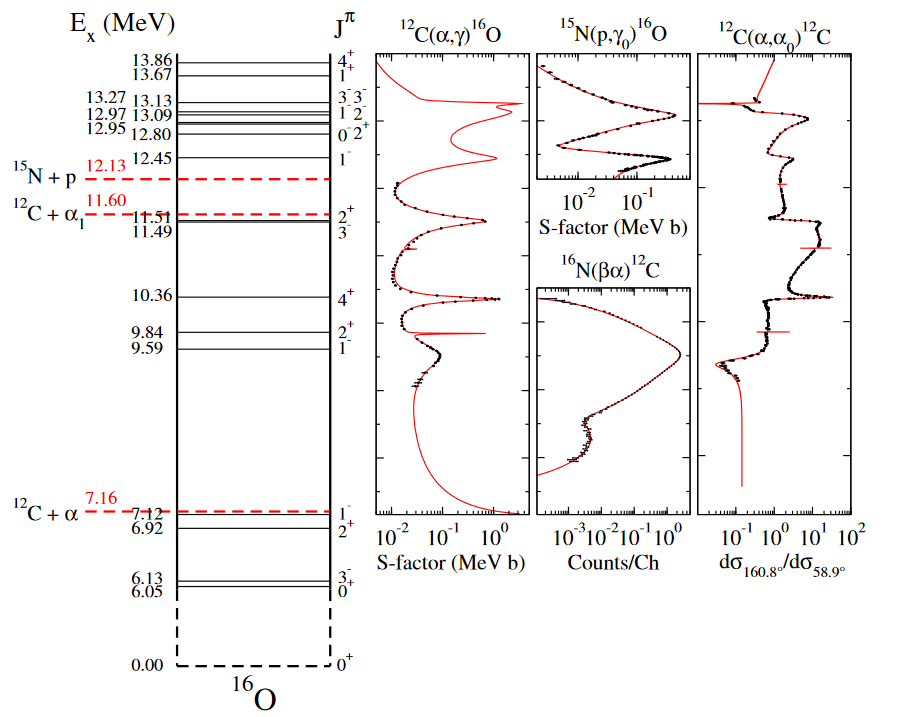
\includegraphics[scale=0.6]{Immagini/0426_lv.png}
	\caption{Livelli energetici dell'ossigeno (a sinistra) e fattore astrofisico (a destra) per le reazioni $\ce{^{12}C}(\alpha,\gamma)\ce{^{16}O}$, $\ce{^{15}N}(p,\gamma)\ce{^{16}O}$ e $\ce{^{12}C}(\alpha,\alpha)\ce{^{12}C}$ (scattering elastico). Sotto i $7.12$ MeV abbiamo stati legati, che non ci interessano perché sottosoglia; per lo stato $1^-$ abbiamo una risonanza larga. I punti sono i dati sperimentali mentre la curva in rosso è un fit \vir{teorico-fenomenologico}.}
	\label{0426_lv}
\end{figure}

\noindent Studiamo le catture che possiamo avere:
\begin{enumerate}[i.]
	\item Cattura diretta, quindi su uno dei 5 stati legati e di conseguenza non risonante. $S=0$ per cui $J_i = \ell_i$ e $\pi_i = (-)^\ell$; per l'ossigeno abbiamo $J^\pi = 0^+,3^-,2^+,1^-$ (dove $0^+$ è preso 2 volte). Ricordiamo che $\ell=0$ non è possibile dal momento che la transizione $0^+\to0^+$ non è permessa dal decadimento $\gamma$.
	\begin{itemize}
		\item[-] $\ell =1$ $1^-\to0^+$ (g.s.) con un $E1$.
		\item[-] $\ell=2$ $2^+\to0^+$ (g.s.) con un $E2$. 
	\end{itemize}
	Ricordiamo che per $\ell\not = 0$ il termine di barriera centrifuga si fa sentire e sopprime in parte la cattura diretta. Per $E1$, inoltre, abbiamo anche un altro problema: per $q\to0$ 
	$$E\lambda \to Z_{eff}^{(\lambda)}\,r_{\alpha\mbox{C}}^\lambda Y_{\lambda \mu}(\hat{r}_{\alpha\mbox{C}})$$
	$$Z_{eff}^{(\lambda)} \equiv Z_\alpha \ppc{\frac{m_{C}}{m_\alpha + m_{C}}}^\lambda + Z_C \ppc{\frac{-m_\alpha}{m_\alpha+m_C}}^\lambda$$
	dove abbiamo definito la carica efficace\index{carica efficace} $Z_{eff}^{(\lambda)}$ (ma non approfondiamo il significato di tale definizione). Allora valutiamo la carica efficacie per $E1$:
	$$Z_{eff}^{(1)} = 2{\frac{m_{C}}{m_\alpha + m_{C}}} - 6 {\frac{m_\alpha}{m_\alpha+m_C}} \stackrel{\ce{C}\sim 3\alpha}{\simeq} 2 \frac{3m_\alpha}{4m_\alpha} - 6 \frac{m_\alpha}{4m_\alpha} = 0$$
	Il termine $E1$ è quindi soppresso. Una spiegazione più elegante di questo fatto è data dal fatto che essendo $Z_{eff}$ molto piccola i nuclei coinvolti saranno tutti circa a isospin nullo: $\ce{^4He} = nn\, pp$ $T_z=0$ e $T=0,1,2$, dove però $T=0$ sarà dominante; ugualmente per $\ce{^12C_6}$ e $\ce{^{16}O_8}$. $E1$ si porta dietro nella corrente la dipendenza dall'isospin secondo il termine in $\tau_z$ (isovettoriale) allora dal momento che $T_i=0\to0=T_f$ è soppressa lo è anche $E1$. In sintesi, $E1\sim E2$ sono paragonabili\footnote{Questo avviene anche per altre reazioni.} %! Sul quaderno ho segnato anche p+d
	e questo comporta che la cattura diretta sia fortemente soppressa.
	\item Cattura risonante soprasoglia, per $E_X = 9.59$ MeV $J^\pi = 1^-$ e $E_X = 9.84$ MeV $J^\pi = 2^+$. Quest'ultima è stretta e non ci interessa; $1^-$ ha invece larghezza $\Gamma=2.4$ MeV (molto larga). Il contributo sarà $E1$ perché la transizione è $1^-\to0^+$ e non abbiamo il problema della soppressione.
	\item Cattura risonante sottosoglia, per $E_X = 7.12$ MeV $J^\pi =1^-$ ($E_R\simeq -45$ keV) e $E_X = 6.92$ MeV $J^\pi =2^+$ ($E_R\simeq -245$ keV). Queste sono responsabili della risalita del fattore astrofisico in Figura \ref{0426_lv} per $E\to0$. Abbiamo quindi $E1$ da $1^-\to0^+$ ed $E2$ da $2^+\to0^+$ con lo stesso ordine di grandezza ($E1\sim E2$).
\end{enumerate}

\paragraph{Teoria ed esperimenti}
Nel 1937 Wheeler fece per la prima volta i conti per questa reazione e propose un \textit{cluster model}\index{cluster model@\textit{cluster model}}\footnote{Modello ripreso di recente.}: si considerano i nuclei come \textit{cluster} di particelle $\alpha$ (che sono particolarmente legate, $B_\alpha = 28$ MeV), per cui $\ce{^{12}C}=3\alpha$ e $\ce{^{16}O}=4\alpha$; l'approssimazione è buona se rimaniamo a basse energie (come quelle di interesse astrofisico).  
%! Ho scritto qualcosa sul fatto che le eccitazioni possono essere viste come "comp." di una molecola e non so se è composizioni o componenti.
L'unica difficoltà del modello è che richiede un potenziale di interazione effettivo $V_{\alpha \alpha}$ e con questo si ha però problemi a riprodurre le risonanze. Il metodo quindi sarebbe anche valido con un ottimo potere predittivo, tuttavia l'accuratezza richiesta dall'astrofisica non è ancora stata raggiunta.\\ 
Anche metodi \textit{ab-initio}\index{Metodo ab-initio@Metodo \textit{ab-initio}} non sono congeniali, dal momento che la teoria per $A=16$ non è affatto semplice. A oggi, la scelta più frequente è il metodo della \textit{Phenomenological} $R$-MATRIX\index{metodo Rmatrix@metodo $R$-MATRIX!Phenomenological}, che però non dà informazioni sulla funzione d'onda.
Si ha quindi in \textit{input} i dati sperimentali e in \textit{output} la stima del fattore astrofisico, di cui riportiamo i risultati in Figura \ref{0426_Se}. Notiamo che per $E_{Gamow} \simeq 300$ keV non ci sono dati e che se i dati per $E1$ sono approssimativamente in accordo tra le varie acquisizioni non si può certo dire lo stesso dei dati per $E2$, per i quali spesso c'è discrepanza anche tra il fit e l'andamento degli stessi. Si ritiene che ciò derivi da una raccolta dati \vir{sporcata} da un \textit{overall factor} di normalizzazione, che si può correggere con misure a risonanza larga. %! che significa?

\begin{figure}[!h]
	\centering
	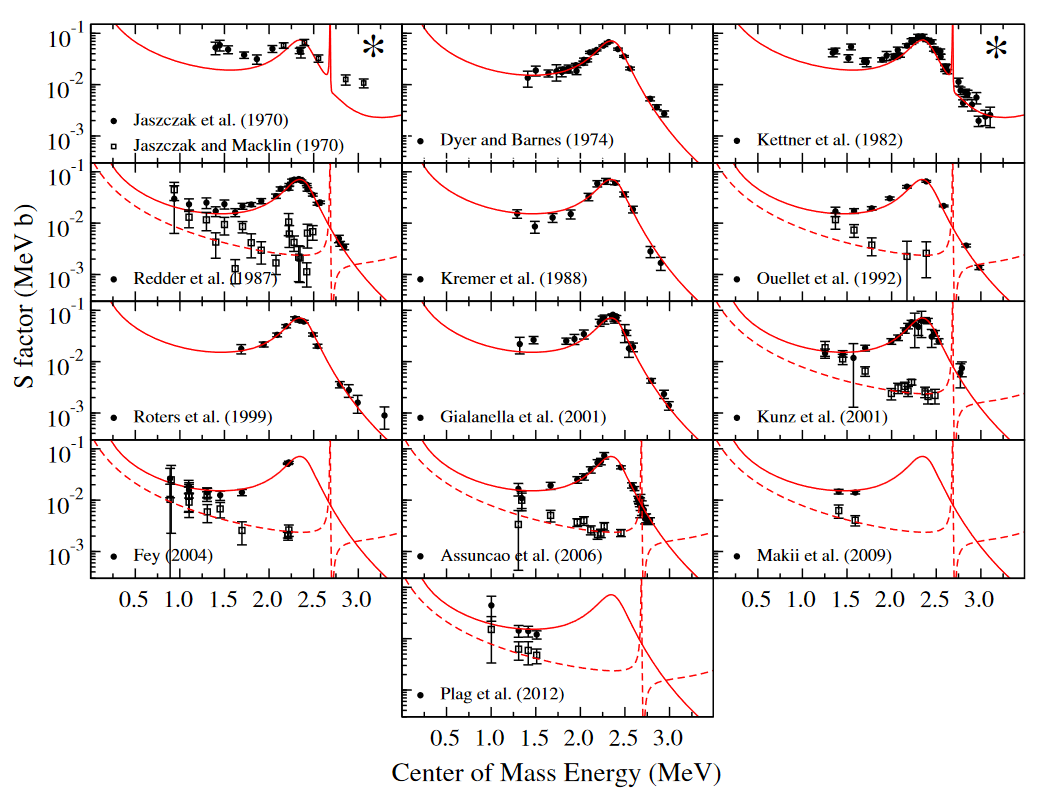
\includegraphics[scale=0.5]{Immagini/0426_SE.png}
	\caption{Risultati per l'analisi con \textit{ph}RM di dati acquisiti in diversi esperimenti dal 1970 al 2012. La linea rossa è il fit ottenuto con \textit{ph}RM: a eccezione dei pannelli con l'asterisco dove è stato misurato $E1+E2$, la linea continua sta per $E1$, mentre quella a tratti per $E2$.}
	\label{0426_Se}
\end{figure}

\noindent Come appunto detto, per l'energia di Gamow non ci sono dati per cui è chiaro come il metodo \textit{ph}RM sia essenziale in questo studio. Nella Figura \ref{0426_storia} riportiamo l'andamento del valore del fattore astrofisico nel tempo al variare del metodo e dell'anno dei vari esperimenti e analisi. La stima più recente dà:
$$S(300\unit{keV}) = (140\pm 21)\unit{keV b}$$
L'incertezza è del 20\% circa (dovuta per esempio a inconsistenze tra set di dati spetimentali) e dev'essere ridotta al 10\%.

\begin{figure}[!h]
	\centering
	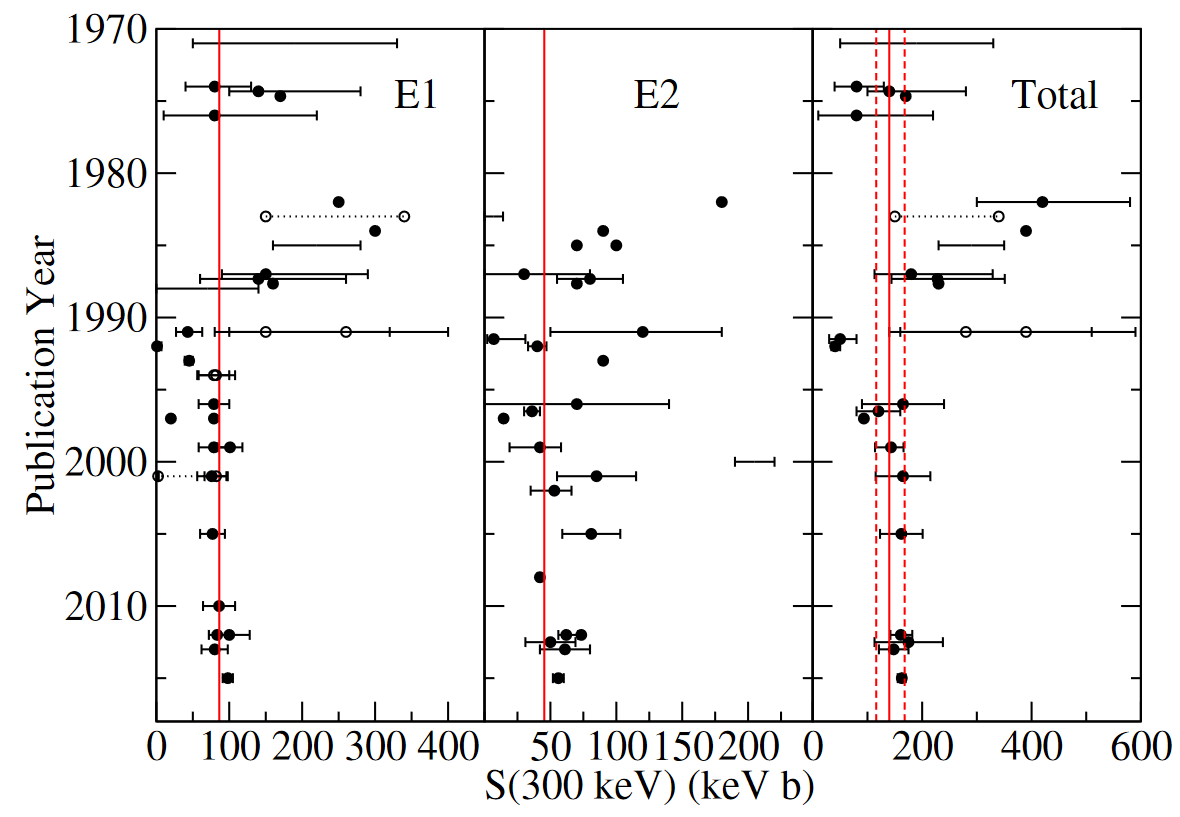
\includegraphics[scale=0.4]{Immagini/0426_storia.png}
	\caption{Andamento del valore del fattore astrofisico al picco di Gamow nel tempo al variare della pubblicazione su tale studio: la linea rossa rappresenta il valore ottenuto con \textit{ph}RM.}
	\label{0426_storia}
\end{figure}

\noindent L'obiettivo di LUNA MV\esperimento{LUNA!LUNA MV} e di altri esperimenti come ERNA\esperimento{ERNA}\footnote{ERNA vuole ottenere la misura con il \textit{recoil separetion method}. Le misure indicate con il nome Gialanella et al. in Figura \ref{0426_Se} sono state ottenute con ERNA.} e all'estero DRAGON\esperimento{DRAGON} è proprio la misura di questa reazione.


